\documentclass[journal]{IEEEtran}
\usepackage{amsmath,amssymb}
\usepackage{graphicx}
\usepackage{booktabs}
\usepackage{cite}
\usepackage{tikz}
\usetikzlibrary{positioning,arrows.meta,shapes.geometric,fit,calc}
\usepackage[hidelinks]{hyperref}

\definecolor{slate}{HTML}{3B5B7E}
\definecolor{navy}{HTML}{24405F}
\definecolor{dblue}{HTML}{2C5D8F}
\definecolor{amber}{HTML}{C46A1D}
\definecolor{paleblue}{HTML}{E4ECF5}
\definecolor{paleamber}{HTML}{F8EBDD}
\definecolor{softgrey}{HTML}{F4F6F9}

\begin{document}

\title{LLM Hallucination Detection Using EigenScore on Internal States for Reliable Question Answering}

\author{Prapti Chotaliya(202411030), Aayaan Ali Khan(202411001), Shlok Bhavsar(202411018)\\
Under the guidance of Dr.~Venkata Phanikrishna\\
Indian Institute of Information Technology, Vadodara - International Campus Diu}

\maketitle

\begin{abstract}
This paper presents a hallucination detection system that flags likely-wrong answers of a large language model (LLM) without access to the correct answer. The system asks the model the same question several times and measures how much the resulting answers disagree, not in their words but in the model's internal representation of each answer. For every answer, the hidden state of the last token at the middle layer of Llama-2-7B is extracted, the covariance between the sampled answers is computed, and the average logarithm of its eigenvalues, called the EigenScore, is used as the hallucination score. The system runs on an 8~GB laptop GPU through 4-bit quantisation, selective hidden-state capture and batched sampling. On 250 questions from the CoQA dataset, the system achieves an AUROC of 83.5\%, the highest among five detection methods evaluated on the same answers. Overall, the system provides a lightweight, answer-key-free and deployable mechanism for screening unreliable LLM outputs.
\end{abstract}

\begin{IEEEkeywords}
Hallucination Detection, Large Language Models, EigenScore, Internal States, Covariance, Eigenvalues, Llama-2, AUROC, 4-bit Quantisation.
\end{IEEEkeywords}

\section{Introduction}
\IEEEPARstart{L}{arge} language models (LLMs) are being rapidly adopted in chatbots, search assistants, tutoring systems and business automation. A persistent problem is \emph{hallucination}: the model produces a fluent and confident answer that is factually wrong. Because a wrong answer is written in the same tone as a correct one, a user cannot tell the two apart from the text alone. Example: when asked ``In which year did the bridge open?'', a model may reply ``The bridge opened in 1928'' with full confidence even if the correct year is different.

In deployment, the correct answer is not available, so the output cannot simply be checked against a reference. Hence, this paper presents a system that assigns a \emph{hallucination score} to every answer using only the model itself. The key observation is that when a model knows an answer, repeated samples agree with each other; when it is guessing, they scatter. Instead of comparing the sampled answers by their words, the system compares the model's \emph{internal states}, the vectors the network computes while producing each answer, which capture meaning rather than surface form.

The system uses Llama-2-7B as the backbone, reads the middle-layer hidden state of each sampled answer, and summarises the spread of these vectors with the eigenvalues of their covariance matrix (the EigenScore~\cite{chen2024inside}). It is engineered to run on a consumer laptop GPU with 8~GB of memory and is evaluated on the CoQA question answering dataset~\cite{reddy2019coqa}.

\section{Challenges}
With the rapid growth of LLM-based applications, the quality of generated responses is steadily improving, yet the responses cannot be fully trusted. The following challenges remain:
\begin{itemize}
\item \textbf{Confident Hallucinations:} Wrong answers are produced in the same fluent and assertive style as correct ones, so no signal is visible in the text itself.
\item \textbf{No Answer Key at Run Time:} In real use, the reference answer is unknown. A practical detector must work from the model and the question alone.
\item \textbf{Semantic Variability:} The same meaning can be expressed in many ways. ``1932'' and ``in nineteen thirty-two'' share no words yet mean the same, so word-level comparison misjudges agreement.
\item \textbf{Limited Hardware:} A 7-billion-parameter model needs about 13.5~GB in 16-bit precision, which exceeds the memory of common laptop GPUs.
\end{itemize}

\section{Limitations}
Detectors based on output probabilities look at one answer at a time and cannot tell confident errors from confident facts. Detectors that compare several answers by their text depend on wording, so paraphrases appear as disagreement and different wrong answers with shared words appear as agreement. Both families discard the information that is still present inside the network. In addition, storing all hidden layers for every generated token is memory-intensive, which makes internal-state methods difficult to run on small GPUs.

\section{Existing Approach}
Several methods have been used to estimate whether an LLM answer is reliable, ranging from simple probability-based scores to comparison of multiple sampled answers. These approaches provide only a partial solution.
\begin{itemize}
\item \textbf{Perplexity:} Measures how surprised the model is by its own answer, based on token probabilities. It is simple, but a model can be confidently wrong, and a low-perplexity answer is not necessarily correct.
\item \textbf{Length-Normalised Entropy (LN-Entropy):} Averages the uncertainty of several sampled answers, normalised by their length~\cite{malinin2021uncertainty}. It uses more than one sample but still relies only on token probabilities.
\item \textbf{Lexical Similarity:} Computes the average ROUGE-L overlap~\cite{lin2004rouge} between sampled answers. It captures agreement, but only at the level of words, and fails for paraphrases.
\item \textbf{Energy Score:} An out-of-distribution score derived from the output logits~\cite{liu2020energy}. It was designed for classification tasks and is weakly related to factual correctness.
\end{itemize}

\begin{figure}[!t]
\centering
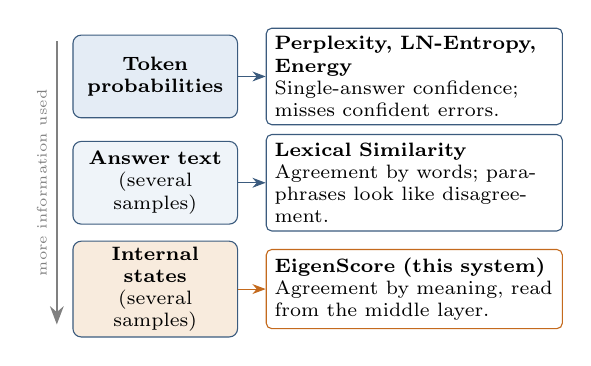
\begin{tikzpicture}[font=\scriptsize,
  box/.style={draw=slate,rounded corners=2pt,fill=white,align=left,text width=3.55cm,inner sep=3pt},
  lvl/.style={draw=slate,fill=#1,rounded corners=3pt,align=center,text width=1.95cm,minimum height=1.05cm,inner sep=2pt}]
\node[lvl=paleblue] (a) at (0,0) {\textbf{Token}\\\textbf{probabilities}};
\node[lvl=paleblue!60] (b) at (0,-1.35) {\textbf{Answer text}\\(several samples)};
\node[lvl=paleamber] (c) at (0,-2.7) {\textbf{Internal states}\\(several samples)};
\node[box,right=0.35cm of a] (ta) {\textbf{Perplexity, LN-Entropy, Energy}\\ Single-answer confidence; misses confident errors.};
\node[box,right=0.35cm of b] (tb) {\textbf{Lexical Similarity}\\ Agreement by words; paraphrases look like disagreement.};
\node[box,right=0.35cm of c,draw=amber] (tc) {\textbf{EigenScore (this system)}\\ Agreement by meaning, read from the middle layer.};
\draw[-{Stealth},slate] (a)--(ta); \draw[-{Stealth},slate] (b)--(tb); \draw[-{Stealth},amber] (c)--(tc);
\draw[-{Stealth},thick,gray] (-1.25,0.45)--node[midway,rotate=90,above,font=\tiny]{more information used} (-1.25,-3.15);
\end{tikzpicture}
\caption{Existing approaches for LLM answer reliability and the signal each one uses.}
\label{fig:existing}
\end{figure}

\section{Proposed Methodology}
\subsection{System Overview}
The proposed system acts as a verification layer placed after any open LLM. For each question it outputs one number, the hallucination score; a higher score indicates a more likely wrong answer. The workflow is defined through six sequential steps:
\begin{itemize}
\item \textbf{User Question:} The system receives a question, together with its context passage in the case of CoQA.
\item \textbf{Multiple Sampling:} The LLM generates $K=10$ answers with temperature $0.5$, top-$p$ $0.99$ and top-$k$ $10$, so that uncertainty in the model shows up as variation between answers.
\item \textbf{Embedding Extraction:} For each answer $i$, the hidden state of its last token at layer 16 of the 32-layer model is read through a forward hook, giving a vector $z_i\in\mathbb{R}^{4096}$. The last token is used because the model reads left to right, so this token has ``seen'' the whole answer. The middle layer is used because early layers encode surface word patterns, while the final layers specialise in predicting the next word.
\item \textbf{Covariance Computation:} The $K$ vectors form a matrix $Z\in\mathbb{R}^{K\times 4096}$, and the covariance between answers is computed:
\begin{equation}
C=\operatorname{cov}(Z)\in\mathbb{R}^{K\times K}
\end{equation}
where:
\begin{itemize}
\item[--] $C$ = covariance matrix between the $K$ answers
\item[--] $Z$ = matrix whose rows are the answer embeddings $z_i$
\item[--] $K$ = number of sampled answers ($10$)
\end{itemize}
\item \textbf{Eigenvalue Decomposition:} The eigenvalues $\lambda_1,\dots,\lambda_K$ of the regularised covariance $C+\alpha I$ are obtained by singular value decomposition, where $\alpha=10^{-3}$ keeps the matrix full rank.
\item \textbf{Hallucination Score:} The EigenScore is the average logarithm of the eigenvalues:
\begin{equation}
E=\frac{1}{K}\sum_{i=1}^{K}\log_{10}\lambda_i=\frac{1}{K}\log_{10}\det\left(C+\alpha I\right)
\end{equation}
where:
\begin{itemize}
\item[--] $E$ = EigenScore (hallucination score)
\item[--] $\lambda_i$ = $i$-th eigenvalue of $C+\alpha I$
\item[--] $\alpha$ = regularisation constant ($10^{-3}$)
\item[--] $I$ = $K\times K$ identity matrix
\end{itemize}
\end{itemize}
When the answers agree, the vectors nearly coincide, one eigenvalue dominates and the rest collapse towards $\alpha$, giving a low score. When the answers disagree, the vectors spread in many directions, several eigenvalues are large, and the score is high.

\subsection{Model Architecture}
The architecture is divided into four key components:
\begin{itemize}
\item \textbf{Backbone LLM:} Llama-2-7B~\cite{touvron2023llama2} with 32 decoder layers and a hidden size of 4096, loaded with 4-bit NF4 weights~\cite{dettmers2023qlora} through the \texttt{transformers}~\cite{wolf2020transformers} and \texttt{bitsandbytes} libraries. This reduces the weight memory from 13.5~GB to about 3.9~GB.
\item \textbf{Embedding Capture Hook:} A forward hook on layer 16 stores only the last-token vector of each answer, instead of all 33 hidden states for every token.
\item \textbf{Scoring Module:} Computes the covariance, eigenvalues and EigenScore with \texttt{torch.cov}, \texttt{np.linalg.svd} and \texttt{np.mean(np.log10(}$\lambda$\texttt{))}.
\item \textbf{Feature Clipping (optional):} A hook on layer 31 clamps each of the 4096 neurons to its normal range during generation, to reduce overconfident activations:
\begin{equation}
\mathrm{FC}(h)=\min\left(\max\left(h,\,h_{\min}\right),\,h_{\max}\right)
\end{equation}
where:
\begin{itemize}
\item[--] $h$ = activation of one neuron for the current token
\item[--] $h_{\min}$, $h_{\max}$ = 0.2th and 99.8th percentiles of that neuron
\item[--] percentiles are estimated from a memory bank of the last $3000$ token activations
\end{itemize}
\end{itemize}

\subsection{Implementation Process}
The system is implemented in Python with PyTorch. Three engineering measures allow the full pipeline to run on an NVIDIA RTX 4060 laptop GPU with 8~GB of memory:
\begin{itemize}
\item 4-bit NF4 quantisation of the model weights (13.5~GB $\rightarrow$ 3.9~GB).
\item Selective capture: only the layer-16 last-token vector is stored, which avoids running out of memory on long CoQA passages.
\item Batched sampling: the 10 answers are generated two at a time over five passes and pooled before scoring, so the score always uses all 10 answers.
\end{itemize}
Correctness of the implementation is verified by eight automated unit tests (8/8 pass), including a check of the clipping thresholds against \texttt{numpy.percentile}, a check that pooled batching gives the same score as a single pass, and a check that selective capture gives the same embedding as the full hidden-state path.

\subsection{Evaluation Strategy}
To measure how well the score separates correct from wrong answers, each generated answer is labelled correct when its ROUGE-L overlap with the reference answer exceeds $0.5$, and wrong otherwise. The score is then evaluated with the area under the ROC curve (AUROC), computed with \texttt{scikit-learn}:
\begin{equation}
\mathrm{AUROC}=P\left(E_{\text{wrong}}>E_{\text{correct}}\right)
\end{equation}
where $E_{\text{wrong}}$ and $E_{\text{correct}}$ are the scores of a randomly chosen wrong and correct answer. Random guessing gives $50\%$ and a perfect detector gives $100\%$.

\subsection{Decision Logic}
After scoring, the output is interpreted with a threshold $\tau$ chosen on validation data according to the application's tolerance for risk:
\begin{itemize}
\item If $E>\tau$ $\rightarrow$ flag the answer as a likely hallucination (warn the user, abstain, or route to retrieval or a human).
\item If $E\le\tau$ $\rightarrow$ return the answer normally.
\end{itemize}
This ensures that unreliable answers are flagged before they reach the user.

\begin{figure}[!t]
\centering
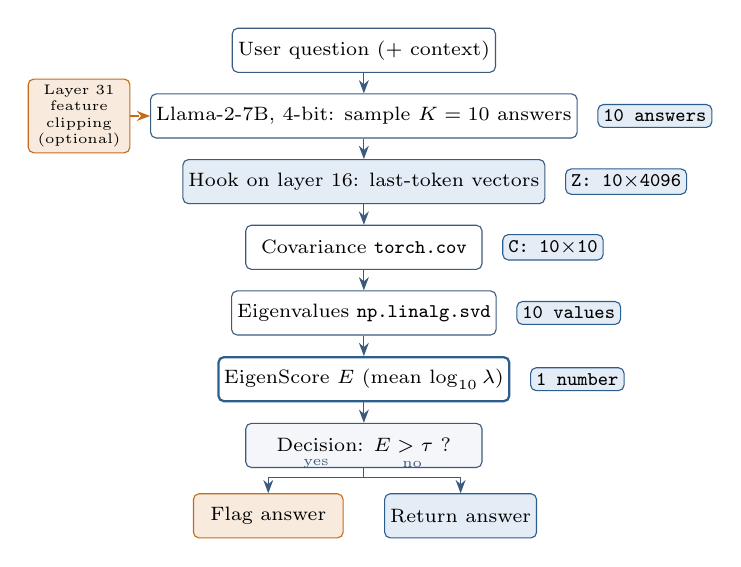
\begin{tikzpicture}[font=\scriptsize, node distance=0.26cm,
  st/.style={draw=slate,rounded corners=2pt,fill=white,minimum width=3.0cm,minimum height=0.56cm,align=center,inner sep=2pt},
  dm/.style={draw=dblue,fill=paleblue,rounded corners=2pt,font=\scriptsize\ttfamily,inner sep=2pt},
  ar/.style={-{Stealth},slate}]
\node[st] (q) {User question (+ context)};
\node[st,below=of q] (g) {Llama-2-7B, 4-bit: sample $K=10$ answers};
\node[st,below=of g,fill=paleblue] (h) {Hook on layer 16: last-token vectors};
\node[st,below=of h] (c) {Covariance \texttt{torch.cov}};
\node[st,below=of c] (e) {Eigenvalues \texttt{np.linalg.svd}};
\node[st,below=of e,draw=dblue,thick] (s) {EigenScore $E$ (mean $\log_{10}\lambda$)};
\node[st,below=of s,fill=softgrey] (d) {Decision: $E>\tau$ ?};
\node[st,below left=0.32cm and -1.25cm of d,minimum width=1.9cm,fill=paleamber,draw=amber] (f) {Flag answer};
\node[st,below right=0.32cm and -1.25cm of d,minimum width=1.9cm,fill=paleblue,draw=dblue] (r) {Return answer};
\foreach \a/\b in {q/g,g/h,h/c,c/e,e/s,s/d} \draw[ar] (\a)--(\b);
\draw[ar] (d.south) -- ++(0,-0.12) -| node[pos=0.25,above,font=\tiny]{yes} (f.north);
\draw[ar] (d.south) -- ++(0,-0.12) -| node[pos=0.25,above,font=\tiny]{no} (r.north);
\node[dm,right=0.25cm of g] {10 answers};
\node[dm,right=0.25cm of h] {Z: 10$\times$4096};
\node[dm,right=0.25cm of c] {C: 10$\times$10};
\node[dm,right=0.25cm of e] {10 values};
\node[dm,right=0.25cm of s] {1 number};
\node[st,left=0.25cm of g,minimum width=1.2cm,text width=1.15cm,draw=amber,fill=paleamber,font=\tiny] (fc) {Layer 31\\feature clipping\\(optional)};
\draw[-{Stealth},amber,dashed] (fc)--(g);
\end{tikzpicture}
\caption{Proposed hallucination detection pipeline, with the real tensor sizes used in the experiment.}
\label{fig:pipeline}
\end{figure}

\section{Advantages}
\begin{itemize}
\item \textbf{No Answer Key Required:} The score is computed from the model's own samples, so it can be used at run time on new questions.\\
Example: a chatbot can warn the user about an answer to a question nobody has answered before.
\item \textbf{Meaning-Level Agreement:} Internal states capture semantics, so paraphrased answers are treated as agreeing.\\
Example: ``1932'' and ``in nineteen thirty-two'' have 0\% word overlap but close internal vectors.
\item \textbf{Single, Interpretable Number:} One score per question, with a clear meaning: the spread of the model's answers in its own representation space.
\item \textbf{Runs on Consumer Hardware:} The complete system, including a 7-billion-parameter model, runs within 8~GB of GPU memory, using about 3.9~GB for the model weights.
\item \textbf{Low Overhead Beyond Sampling:} The scoring itself operates on a $10\times10$ matrix, so its cost is negligible compared with generating the answers.
\item \textbf{Model-Agnostic Design:} Any open-weight transformer that exposes its hidden states can be used as the backbone by changing the hooked layer.
\item \textbf{Verified Implementation:} Eight unit tests check the mathematical components and the memory optimisations against reference implementations.
\end{itemize}

\section{Experimental Results and Discussion}
To evaluate the proposed system, Llama-2-7B was run on 250 questions from the CoQA development set with a fixed seed (2023). The model answered 92 questions correctly (36.8\%) and 158 incorrectly (63.2\%). Five scores were computed from the same generated answers, and Table~\ref{tab:results} presents their detection performance.

\begin{table}[!t]
\centering
\caption{Detection Performance on 250 CoQA Questions}
\label{tab:results}
\begin{tabular}{@{}lcc@{}}
\toprule
\textbf{Method} & \textbf{AUROC (\%)} & \textbf{AUROC with FC (\%)}\\
\midrule
\textbf{EigenScore (proposed)} & \textbf{83.5} & \textbf{82.5}\\
Lexical Similarity & 80.5 & 79.3\\
LN-Entropy & 77.5 & 77.3\\
Perplexity & 72.3 & 71.4\\
Energy & 54.7 & 53.1\\
\midrule
\multicolumn{3}{@{}l}{\emph{Time per question (10 answers + score): $\approx$ 6 s}}\\
\multicolumn{3}{@{}l}{\emph{GPU memory for model weights: $\approx$ 3.9 GB of 8 GB}}\\
\bottomrule
\end{tabular}
\end{table}

\noindent\textbf{A. Quantitative Analysis}

The proposed system achieved an AUROC of \textbf{83.5\%}: given one wrong and one correct answer chosen at random, the EigenScore is higher for the wrong answer in 83.5\% of cases. With feature clipping enabled, the AUROC was \textbf{82.5\%}. Each question, including the generation of 10 answers and scoring, took about 6 seconds, and the model weights used about 3.9~GB of GPU memory.

\noindent\textbf{B. Comparative Insights}

The EigenScore achieved the highest AUROC among all five methods evaluated on the same answers, improving on the strongest alternative, Lexical Similarity, by 3.0 points. A paired bootstrap with 10\,000 resamples over questions gives a difference of $+2.9$ points with a 95\% confidence interval of $[-0.6,\,+6.5]$, positive in 95\% of resamples. This improvement mainly comes from three factors:
\begin{itemize}
\item \textbf{Internal representations} compare answers by meaning rather than by shared words.
\item \textbf{Eigenvalue-based spread} uses the full geometry of all 10 answers instead of averaging pairwise similarities.
\item \textbf{Middle-layer embeddings} carry richer semantic information than the output probabilities used by Perplexity, LN-Entropy and Energy.
\end{itemize}

\noindent\textbf{C. Observations}
\begin{itemize}
\item Methods that use multiple samples (EigenScore, Lexical Similarity, LN-Entropy) clearly outperform single-answer scores (Perplexity, Energy).
\item The Energy score is close to chance (54.7\%), confirming that logit-based out-of-distribution scores are not suited to factual correctness.
\item Feature clipping was verifiably active (0.29\% of activations clipped), but its effect, $-1.0$ point with a 95\% interval of $[-4.7,\,+2.6]$, cannot be resolved with 250 questions.
\item Limitations: each question needs 10 generations; the method requires access to hidden states, so it applies to open models rather than closed APIs; it detects but does not correct errors; and the evaluation covers one dataset.
\end{itemize}

\noindent\textbf{D. Future Directions}
\begin{itemize}
\item \textbf{Multi-layer EigenScore:} combine a band of middle layers into one score instead of a single hand-picked layer.
\item \textbf{Token-confidence fusion:} join the spread score with word-level confidence to catch answers that are consistently wrong.
\item \textbf{Adaptive sampling:} stop sampling early when the first answers clearly agree, reducing cost below 10 generations.
\end{itemize}

\section{Conclusion}
This paper presented a hallucination detection system for LLMs that uses the model's internal states. By sampling several answers, reading their middle-layer embeddings and summarising their spread with the eigenvalues of the covariance matrix, the system produces one interpretable hallucination score per question without needing the correct answer. Through 4-bit quantisation, selective hidden-state capture and batched sampling, the complete system runs on an 8~GB laptop GPU. On 250 CoQA questions it achieved an AUROC of 83.5\%, the best among the five methods evaluated. This work provides an effective and practical solution for screening unreliable LLM answers, supporting safer deployment of question answering and conversational AI systems.

\begin{thebibliography}{9}
\bibitem{chen2024inside} C. Chen, K. Liu, Z. Chen, Y. Gu, Y. Wu, M. Tao, Z. Fu, and J. Ye, ``INSIDE: LLMs' Internal States Retain the Power of Hallucination Detection,'' in Proc. Int. Conf. Learning Representations (ICLR), 2024.
\bibitem{reddy2019coqa} S. Reddy, D. Chen, and C. D. Manning, ``CoQA: A Conversational Question Answering Challenge,'' Trans. Assoc. Comput. Linguistics, vol. 7, pp. 249--266, 2019.
\bibitem{touvron2023llama2} H. Touvron et al., ``Llama 2: Open Foundation and Fine-Tuned Chat Models,'' arXiv:2307.09288, 2023.
\bibitem{dettmers2023qlora} T. Dettmers, A. Pagnoni, A. Holtzman, and L. Zettlemoyer, ``QLoRA: Efficient Finetuning of Quantized LLMs,'' in Proc. NeurIPS, 2023.
\bibitem{malinin2021uncertainty} A. Malinin and M. Gales, ``Uncertainty Estimation in Autoregressive Structured Prediction,'' in Proc. ICLR, 2021.
\bibitem{lin2004rouge} C.-Y. Lin, ``ROUGE: A Package for Automatic Evaluation of Summaries,'' in Text Summarization Branches Out, ACL Workshop, 2004.
\bibitem{liu2020energy} W. Liu, X. Wang, J. Owens, and Y. Li, ``Energy-based Out-of-distribution Detection,'' in Proc. NeurIPS, 2020.
\bibitem{wolf2020transformers} T. Wolf et al., ``Transformers: State-of-the-Art Natural Language Processing,'' in Proc. EMNLP: System Demonstrations, 2020.
\end{thebibliography}

\end{document}
